\chapter{Roman Units}
The ancient units of measurement were built upon the Greek system with influences from Egyptian, Hebrew and Mesopotamian influences. The Roman units were
comparatively consistent and well documented.

\subsection{Lengths}

\begin{marginfigure}
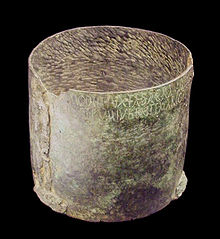
\includegraphics[width=\linewidth]{./graphics/modius}
\caption{Bronze modius measure (4th cent. AD) with inscription acknowledging Imperial regulation of weights and measures.}
\end{marginfigure}


The basic unit of Roman linear measurement was the \textit{pes} or Roman foot. Investigation of its relation to the English foot goes back at least to 1647, when John Greaves published his \textit{Discourse on the Romane foot}. Greaves visited Rome in 1639, and measured, among other things, the foot measure on the tomb of Titus Statilius Aper, that on the statue of Cossutius formerly in the gardens of Angelo Colocci, the congius of Vespasian previously measured by Villalpandus, a number of brass measuring-rods found in the ruins of Rome, the paving-stones of the Pantheon and many other ancient Roman buildings, and the distance between the milestones on the Appian Way. He concluded that the Cossutian foot was the "true" Roman foot, and reported these values compared to the iron standard of the English foot in the Guildhall in London.



\SetConversion{pes}{ft}{0.967}
\SetConversion{pes}{in}{294.7}

\SetConversion{digitus}{mm}{18.5}
\SetConversion{uncia}{inch}{0.971}

\SetConversion{palmus}{digitus}{0.25}
\SetConversion{palmus}{mm}{74}
\SetConversion{palmus}{pes}{0.25}

\SetInBetween{$\to$}

\begin{table}[htbp]
\begin{conversiontable}
\convert{1}{pes}{ft}\\
\convert{1}{palmus}{pes}\\
\convert{1}{uncia}{inch}\\
\convert{1}{palmus}{mm}\\
\convert{1}{inch}{uncia}\\
\end{conversiontable}
\caption{Roman length units.}

\end{table}

As starting measurements from the smaller units proved futile, Greaves changed his plan to measure the distance between \textit{milestones}. These milestones in the \textit{Appian} way, the Romans divided and distinguished their miles; and which occasioned those phrase, \textit{ad primum}, ad quartum, ad centesimum lpidem, and the ike.


Greaves writes:


\begin{quotation}
Wherefore having received small satisfaction from the writings of the ancients, and not much better from the imperfect designations of the \textit{Roman} foot by modern authors, I proposed to my self in my travels abroad these ways, which no
reasonable man must approve of. And those were, first to examine as many ancient measures an monuments in \textit{Italy}, and other parts as it was possible; and secondly, to compare these with as many standards and orginals, as I could procure the sight of. And last of all, to transmit both these and them to posterity, I exactly measured some of the most lasting monuments of the ancients. To this purpose, in the year 1639 I went to Italy, to view asthe other antiquities of the Romans, so especially those of weights and measures; and to take them with as much exactness as it was possible, I carried instruments with me made by the best artizans. 

\end{quotation}

We can only guess, how long the trips and the study took, but it resulted in a publication who survived and forms the basis of the following table:
\medskip

\begin{tabular}{p{8cm}l}
\toprule
Measurement & ft\\
\midrule
Roman foot on the monument of Statilius & .967\\
The foot on the monument of Statilius in Rome & .972\\
The foot of Villalpandus, deduced from the congius of Vespasian & .986\\ 
The Greek foot & 1.007\\
The Venetian foot &1.162\\
The Rhineland foot, or that of Snellius &1.033\\
The derah or cubit at Cairo in Egypt &1.824\\
The Persian arist &3.197\\
The greater Turkish pike at Constantinople & 2.2\\
The braccio at Florence & 1.913\\

\bottomrule
\end{tabular}
\medskip

Greaves investigation into measures and standards did not stop here, he also investigated the cubit and the Denarius, which was a weight measure.

\section{Areas}

The ordinary units of area are shown in Table~\ref{tbl:romanareaunits}

\begin{table}[htbp]
\small\raggedright
\begin{tabular}{p{2.5cm}lll}
\toprule
Roman unit &   Equal to & Metric equivalent & Remarks\\
\midrule
pes  quadratus &  &0.0876\si{\square\meter} & square foot\\
scrupulum or decempeda quadrata & & &\\
actus simplex & & &\\
uncia         & & &\\
clima         & & &\\
actus quadratus or acnua & & &\\
jugerum                  & & &\\
heredium                 & & &\\
centuria                 & & &\\
saltus                   & & &\\
\bottomrule
\end{tabular}

\caption{Roman units of area}
\label{tbl:romanareaunits}

\end{table}


Of interest ws the \textit{jugerum} which was \SI{0.25}{ha}. It measured 240 pedes (Roman feet) or 71.0 m in length and 120 pedes or 35.5 m in breadth, containing therefore 28,800 pedes quadratum (Colum. R. R. v.i \S 6; Quintil. i.18). That is 0.623 acre or \aunit{0.25}{ha}.

It was the double of the Actus Quadratus, and from this circumstance, according to some writers, it derived its name (Varro, L. L. v.35, M\"uller, R. R. i.10). [Actus.] It seems probable that, as the word was evidently originally the same as jugum, a yoke, and as actus, in its original use, meant a path wide enough to drive a single beast along, that jugerum originally meant a path wide enough for a yoke of oxen, namely, the double of the actus in width; and that when actus quadratus was used for a square measure of surface, the jugerum, by a natural analogy, became the double of the actus quadratus; and that this new meaning of it superseded its old use as the double of the single actus.

Pliny (Book XVIII. Chapter 3) states "That portion of land used to be known as a "jugerum," which was capable of being ploughed by a single "jugum," or yoke of oxen, in one day; an "actus" being as much as the oxen could plough at a single spell, fairly estimated, without stopping. This last was one hundred and twenty feet in length; and two in length made a jugerum." (The Natural History, Pliny the Elder, translated by John Bostock, M.D., F.R.S. H.T. Riley, Esq., B.A. London. Taylor and Francis, Red Lion Court, Fleet Street. 1855).

The uncial division as was applied to the jugerum, its smallest part being the scrupulum of 100 sq ft or 9.2 m². Thus, the jugerum contained 288 scrupula (Varro, R. R. l.c.). The jugerum was the common measure of land among the Romans. Two jugera formed an heredium, a hundred heredia a centuria, and four centuriae a saltus. These divisions were derived from the original assignment of landed property, in which two jugera were given to each citizen as heritable property (Varro, l.c.; Niebuhr, Hist. of Rome, vol. ii pp156, \&c., and Appendix ii.).

Other units of area described by Columella in his De Re Rustica include the porca of 180 × 30 Roman feet (about \SI{473}{\square\meter} used in Hispania Baetica and the Gallic candetum or cadetum of \SI{100}{feet} in the city or 150 in the country. Columella also gives uncial divisions of the jugerum, tabulated by the anonymous translator of the 1745 Millar edition as follows:

